\documentclass[12pt,oneside]{report}
\usepackage[utf8]{inputenc}
\usepackage{graphicx}
\graphicspath{ {images/} }
\usepackage{caption}
\usepackage{subcaption}
\usepackage[a4paper,top=38mm,left=38mm,right=25mm,bottom=25mm]{geometry}
\usepackage{fancyhdr}
\usepackage{setspace}

\usepackage{multicol}
\usepackage{tabularx}
\usepackage{acronym}
\usepackage{lastpage}
\usepackage[titletoc]{appendix}
\usepackage{listings}
\usepackage[hyphens]{url}
\usepackage[hidelinks]{hyperref}
\hypersetup{breaklinks=true}
\urlstyle{same}
% Macros for title, author, abstract, etc.
\newcommand \thesistitle{Title of my Thesis}

\newcommand \degreename{Master of Science}

% Use the wording given in the official list of degrees awarded by UCI:
% http://www.rgs.uci.edu/grad/academic/degrees_offered.htm
\newcommand \degreefield{eHealth}

% Your name as it appears on official UCI records.
\newcommand \authorname{Firstname Lastname}

% Use the full name of each committee member.
\newcommand \committeechair{Dr. First Supervisor}
\newcommand \othercommitteemembers
{
  Dr. Second Supervisor\\
  Dr. Third Supervisor\\
  Dr. Fourth Supervisor
}

\newcommand \degreeyear{YEAR}

\newcommand \degreemonth{MONTH}

\newcommand \univname{McMaster University}

\newcommand{\HRule}{\rule{\linewidth}{0.5mm}}

\newcommand \copyrightdeclaration
{
  {\copyright} {\Degreeyear} \Authorname
}


% The dedication page is optional.
\newcommand \dedications
{
  This is dedicated to http://nuchange.ca
}


\newcommand \acknowledgments
{
  Foremost, I would like to express my gratitude to the person who created this LaTeX template. 

\noindent
My teachers 

\noindent
My friends 

\noindent
My batch mates 

\noindent
My survey participants

\noindent
My colleagues 

\noindent
My parents 

\noindent
My wife 


\noindent
And to all others .


}


% Some custom commands for your list of publications and software.
\newcommand{\mypubentry}[3]{
  \begin{tabular*}{1\textwidth}{@{\extracolsep{\fill}}p{4.5in}r}
    \textbf{#1} & \textbf{#2} \\ 
    \multicolumn{2}{@{\extracolsep{\fill}}p{.95\textwidth}}{#3}\vspace{6pt} \\
  \end{tabular*}
}
\newcommand{\mysoftentry}[3]{
  \begin{tabular*}{1\textwidth}{@{\extracolsep{\fill}}lr}
    \textbf{#1} & \url{#2} \\
    \multicolumn{2}{@{\extracolsep{\fill}}p{.95\textwidth}}
    {\emph{#3}}\vspace{-6pt} \\
  \end{tabular*}
}

% Include, at minimum, a listing of your degrees and educational
% achievements with dates and the school where the degrees were
% earned. This should include the degree currently being
% attained. Other than that it's mostly up to you what to include here
% and how to format it, below is just an example.
\newcommand \runninghead
{
Running head here.
}

\newcommand \thesisabbr{
	%\Huge
%List Of Acronyms	\\
%\normalsize
\textbf{DAD} - Discharge Abstract Database \\
\textbf{HMDB} - Hospital Morbidity Database  \\

}

% The abstract should not be over 350 words, although that's
% supposedly somewhat of a soft constraint.
\newcommand \thesisabstract
{
  This is my abstract. Please visit http://nuchange.ca for more details

 

}



	\pagestyle{fancy}
	\fancyhead{}
	\fancyhead[RO,LE]{\runninghead}
	\fancyfoot{}
	\fancyfoot[LE,RO]{\thepage}
	\fancyfoot[LO,CE]{Chapter \thechapter}
	\fancyfoot[CO,RE]{\authorname}
	\renewcommand{\headrulewidth}{0.4pt}
	\renewcommand{\footrulewidth}{0.4pt}
	


%-----------------------------------------------

\usepackage{apacite}
\usepackage{etoolbox}
\usepackage{environ}

\newtoggle{bibdoi}
\newtoggle{biburl}
\makeatletter

\undef{\APACrefURL}
\undef{\endAPACrefURL}
\undef{\APACrefDOI}
\undef{\endAPACrefDOI}

\long\def\collect@url#1{\global\def\bib@url{#1}}
\long\def\collect@doi#1{\global\def\bib@doi{#1}}
\newenvironment{APACrefURL}{\global\toggletrue{biburl}\Collect@Body\collect@url}{\unskip\unskip}
\newenvironment{APACrefDOI}{\global\toggletrue{bibdoi}\Collect@Body\collect@doi}{}

\AtBeginEnvironment{thebibliography}{
	\pretocmd{\PrintBackRefs}{%
		\iftoggle{bibdoi}
		{\iftoggle{biburl}{\unskip\unskip doi:\bib@doi}{}}
		{\iftoggle{biburl}{Retrieved from\bib@url}{}}
		\togglefalse{bibdoi}\togglefalse{biburl}%
	}{}{}
}
%-------------------------------

\begin{document}


%Title in itself in a blank page
\begin{titlepage}
    \begin{center}
        \vspace*{3cm}
        \thesistitle \\
    \end{center}
\end{titlepage}

\begin{titlepage}
\begin{center}

\textsc{\LARGE \univname}\\[1.5cm] % University name
\textsc{\Large MSc Thesis}\\[0.5cm] % Thesis type

\HRule \\[0.4cm] % Horizontal line
\begin{doublespacing}
	{\huge \bfseries \thesistitle}\\[0.4cm] % Thesis title
\end{doublespacing}
\HRule \\[1.5cm] % Horizontal line
 
\begin{minipage}{0.4\textwidth}
\begin{flushleft} \large
\emph{Author:}\\
\authorname % Author name - 
\end{flushleft}
\end{minipage}
\begin{minipage}{0.4\textwidth}
\begin{flushright} \large
\emph{Supervisor:} \\
\committeechair % Supervisor name
\end{flushright}
\end{minipage}\\[2cm]
 
\large \textit{A thesis submitted in partial fulfilment of the requirements\\ for the degree of \degreename}\\[0.3cm] % University requirement text
\textit{in}\\[0.4cm]
%\groupname\\\deptname\\[2cm] % Research group name and department name
\degreefield\\[1.8cm] % Research group name and department name

 
{\large \degreemonth - \degreeyear}\\[1.8cm] % Date

{\copyright} {\degreeyear} \authorname
 
\vfill
\end{center}

\end{titlepage}

\begin{titlepage}
 \begin{flushleft}
    McMaster University, Master of Science eHealth (2015) Hamilton, Ontario \\
        \vspace{0.8in}
    TITLE: \thesistitle \\
        \vspace{0.4in}
    AUTHOR: \authorname \\
    \vspace{0.4in}
    SUPERVISORS: \\
    \committeechair\\
    \othercommitteemembers\\
    \vspace{0.4in}
    NUMBER OF PAGES \pageref{LastPage} \\
\end{flushleft}
\end{titlepage}
\doublespacing
\pagenumbering{roman}
\thispagestyle{plain}
\begin{center}
    \vspace{0.9cm}
    \textbf{Abstract}
\end{center}
\thesisabstract

\chapter*{Dedication}
\dedications

  
\chapter*{Acknowledgements}
\acknowledgments




\clearpage                       % Otherwise \pagestyle affects the previous page.
{                                % Enclosed in braces so that re-definition is temporary.
	\pagestyle{empty}              % Removes numbers from middle pages.
	\fancypagestyle{plain}         % Re-definition removes numbers from first page.
	{
		\fancyhf{}%                       % Clear all header and footer fields.
		\renewcommand{\headrulewidth}{0pt}% Clear rules (remove these two lines if not desired).
		\renewcommand{\footrulewidth}{0pt}%
	}
	\tableofcontents
	\thispagestyle{empty}          % Removes numbers from last page.
}


\listoffigures


\listoftables

\chapter*{List Of Acronyms}
\thesisabbr


\clearpage    

\pagenumbering{arabic}	

\chapter{Introduction}
Lorem ipsum dolor sit amet, sed zril discere an. Pri ad mazim choro vituperatoribus, putent fierent ad per, eu ridens scaevola tractatos vix. Cibo vitae et ius, ad agam facilisis duo. Ea vim etiam tation, scaevola constituam referrentur pro id. Pro id equidem tincidunt, eu qui lorem nonumy \cite{pmid19009985,pmid18797088}.

Usu posse mucius consequuntur id, eam ei brute quaestio dissentiet. Nec ad veri oportere indoctum, eum et suas erroribus consectetuer. Meis verterem sapientem ne eos, ei sit porro facer. Aeque cotidieque has eu, an atqui prompta fuisset usu.

An elitr aliquid bonorum nec, porro placerat consectetuer mel at, eam feugait delicata voluptaria ut. Dicat sonet impetus eum cu, id brute veritus inciderint vel. Soluta detraxit eam id. Mea sale choro no.

At pro odio primis definitionem. Cu vis simul sententiae. Sumo regione ut vim, clita vitae scriptorem ex pro, vitae denique nostrum et mei. Fabellas molestiae sea te, cu enim iisque usu. Melius viderer utroque sit id, commune verterem facilisi qui ad. Vim solum euismod ad, no per tibique appetere \cite{pmid18789058}.

Ea omnis elitr consetetur eum. At vel zril phaedrum sensibus, cu inani mucius ullamcorper quo. Ei alienum tacimates interpretaris duo, vim et nulla oratio. Qui molestie detraxit inimicus eu. Elitr noster persius sea ad, justo postea tamquam ne per.

\chapter{Aims and Objectives}

The aim of the study was to examine the following primary research question:



Our hypothesis was:



The study had the following additional secondary objectives:

\begin{itemize}
\item Aim 1
\item Aim 2
\item Aim 3
\item Aim 4
\item Aim 5
\end{itemize}


\chapter{Review of Literature}
\section{The Review}
Lorem ipsum dolor sit amet, sed zril discere an. Pri ad mazim choro vituperatoribus, putent fierent ad per, eu ridens scaevola tractatos vix. Cibo vitae et ius, ad agam facilisis duo. Ea vim etiam tation, scaevola constituam referrentur pro id. Pro id equidem tincidunt, eu qui lorem nonumy.

Usu posse mucius consequuntur id, eam ei brute quaestio dissentiet. Nec ad veri oportere indoctum, eum et suas erroribus consectetuer. Meis verterem sapientem ne eos, ei sit porro facer. Aeque cotidieque has eu, an atqui prompta fuisset usu.

An elitr aliquid bonorum nec, porro placerat consectetuer mel at, eam feugait delicata voluptaria ut. Dicat sonet impetus eum cu, id brute veritus inciderint vel. Soluta detraxit eam id. Mea sale choro no.

At pro odio primis definitionem. Cu vis simul sententiae. Sumo regione ut vim, clita vitae scriptorem ex pro, vitae denique nostrum et mei. Fabellas molestiae sea te, cu enim iisque usu. Melius viderer utroque sit id, commune verterem facilisi qui ad. Vim solum euismod ad, no per tibique appetere.

Ea omnis elitr consetetur eum. At vel zril phaedrum sensibus, cu inani mucius ullamcorper quo. Ei alienum tacimates interpretaris duo, vim et nulla oratio. Qui molestie detraxit inimicus eu. Elitr noster persius sea ad, justo postea tamquam ne per.

\chapter{Materials and Methods}
\section{Section 1}
Lorem ipsum dolor sit amet, sed zril discere an. Pri ad mazim choro vituperatoribus, putent fierent ad per, eu ridens scaevola tractatos vix. Cibo vitae et ius, ad agam facilisis duo. Ea vim etiam tation, scaevola constituam referrentur pro id. Pro id equidem tincidunt, eu qui lorem nonumy \cite{pmid18583808,pmid18388390}.

Usu posse mucius consequuntur id, eam ei brute quaestio dissentiet. Nec ad veri oportere indoctum, eum et suas erroribus consectetuer. Meis verterem sapientem ne eos, ei sit porro facer. Aeque cotidieque has eu, an atqui prompta fuisset usu.


\subsection{Subsection A}

Lorem ipsum dolor sit amet, sed zril discere an. Pri ad mazim choro vituperatoribus, putent fierent ad per, eu ridens scaevola tractatos vix. Cibo vitae et ius, ad agam facilisis duo. Ea vim etiam tation, scaevola constituam referrentur pro id. Pro id equidem tincidunt, eu qui lorem nonumy.

Usu posse mucius consequuntur id, eam ei brute quaestio dissentiet. Nec ad veri oportere indoctum, eum et suas erroribus consectetuer \cite{pmid18713597}. Meis verterem sapientem ne eos, ei sit porro facer. Aeque cotidieque has eu, an atqui prompta fuisset usu \ref{tab:thesisfirsttable}.

\begin{table}[h]
	\centering
\begin{tabular}{|l|l|}
	\hline
	\multicolumn{1}{|c|}{{\bf Score}} & \multicolumn{1}{c|}{{\bf Various Types}} \\ \hline
	Less than 7                       & Type I                                           \\ \hline
	70-120                              & Type II                                          \\ \hline
	130-180                             & Type III                                         \\ \hline
	190-240                             & Type IV                                          \\ \hline
	250-300                             & Type V                                           \\ \hline
	310 and above                      & Type VI                                          \\ \hline
\end{tabular}
	\caption{This is a caption.}	
	\label{tab:thesisfirsttable}	
\end{table}

\subsection{Subsection B}

An elitr aliquid bonorum nec, porro placerat consectetuer mel at, eam feugait delicata voluptaria ut. Dicat sonet impetus eum cu, id brute veritus inciderint vel. Soluta detraxit eam id. Mea sale choro no.

At pro odio primis definitionem. Cu vis simul sententiae. Sumo regione ut vim, clita vitae scriptorem ex pro, vitae denique nostrum et mei. Fabellas molestiae sea te, cu enim iisque usu. Melius viderer utroque sit id, commune verterem facilisi qui ad. Vim solum euismod ad, no per tibique appetere.

Ea omnis elitr consetetur eum. At vel zril phaedrum sensibus, cu inani mucius ullamcorper quo. Ei alienum tacimates interpretaris duo, vim et nulla oratio. Qui molestie detraxit inimicus eu. Elitr noster persius sea ad, justo postea tamquam ne per.





\section{Section 2}

The testing had 2 phases. 
\begin{enumerate}
\item The first testing phase
\item The second phase.
\end{enumerate}
	
\subsection{Subsection 2a}

An elitr aliquid bonorum nec, porro placerat consectetuer mel at, eam feugait delicata voluptaria ut. Dicat sonet impetus eum cu, id brute veritus inciderint vel. Soluta detraxit eam id. Mea sale choro no.

At pro odio primis definitionem. Cu vis simul sententiae. Sumo regione ut vim, clita vitae scriptorem ex pro, vitae denique nostrum et mei. Fabellas molestiae sea te, cu enim iisque usu. Melius viderer utroque sit id, commune verterem facilisi qui ad. Vim solum euismod ad, no per tibique appetere.

Ea omnis elitr consetetur eum. At vel zril phaedrum sensibus, cu inani mucius ullamcorper quo. Ei alienum tacimates interpretaris duo, vim et nulla oratio. Qui molestie detraxit inimicus eu. Elitr noster persius sea ad, justo postea tamquam ne per in Figure \ref{fig:studydesign}.  

\begin{figure}[h!]
	\centering
	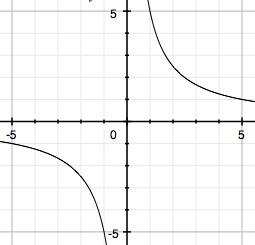
\includegraphics[width=0.9\textwidth, scale=2]{graph3}
	\caption{Study Design}	
	\label{fig:studydesign}	
\end{figure}
 


\subsection{Sample Collection and Statistical Analysis}

The sample size was calculated for a confidence level of 95\% and a confidence interval of 10 using the formula \cite{pmid12653925}: 
Sample Size =	$\frac{Z^2 \times (p) \times (1-p)}{c^2}$


Where:
Z = Z value (e.g. 1.96 for 95\% confidence level) 
p = percentage picking a choice, expressed as decimal (.5 used for sample size needed)
c = confidence interval, expressed as decimal 



\chapter{Results}
\section{Section A}

An elitr aliquid bonorum nec, porro placerat consectetuer mel at, eam feugait delicata voluptaria ut. Dicat sonet impetus eum cu, id brute veritus inciderint vel. Soluta detraxit eam id. Mea sale choro no.

At pro odio primis definitionem. Cu vis simul sententiae. Sumo regione ut vim, clita vitae scriptorem ex pro, vitae denique nostrum et mei. Fabellas molestiae sea te, cu enim iisque usu. Melius viderer utroque sit id, commune verterem facilisi qui ad. Vim solum euismod ad, no per tibique appetere.

Ea omnis elitr consetetur eum. At vel zril phaedrum sensibus, cu inani mucius ullamcorper quo. Ei alienum tacimates interpretaris duo, vim et nulla oratio. Qui molestie detraxit inimicus eu. Elitr noster persius sea ad, justo postea tamquam ne per.

\chapter{Discussion}
Lorem ipsum dolor sit amet, sed zril discere an. Pri ad mazim choro vituperatoribus, putent fierent ad per, eu ridens scaevola tractatos vix. Cibo vitae et ius, ad agam facilisis duo. Ea vim etiam tation, scaevola constituam referrentur pro id \cite{pmid25877226}. Pro id equidem tincidunt, eu qui lorem nonumy.

Usu posse mucius consequuntur id, eam ei brute quaestio dissentiet. Nec ad veri oportere indoctum, eum et suas erroribus consectetuer. Meis verterem sapientem ne eos, ei sit porro facer. Aeque cotidieque has eu, an atqui prompta fuisset usu.

An elitr aliquid bonorum nec, porro placerat consectetuer mel at, eam feugait delicata voluptaria ut. Dicat sonet impetus eum cu, id brute veritus inciderint vel. Soluta detraxit eam id. Mea sale choro no.

At pro odio primis definitionem \cite{pmid20061746}. Cu vis simul sententiae. Sumo regione ut vim, clita vitae scriptorem ex pro, vitae denique nostrum et mei. Fabellas molestiae sea te, cu enim iisque usu. Melius viderer utroque sit id, commune verterem facilisi qui ad. Vim solum euismod ad, no per tibique appetere.

Ea omnis elitr consetetur eum. At vel zril phaedrum sensibus, cu inani mucius ullamcorper quo. Ei alienum tacimates interpretaris duo, vim et nulla oratio. Qui molestie detraxit inimicus eu. Elitr noster persius sea ad, justo postea tamquam ne per \cite{pmid19584464}.


\chapter{Conclusion}
Lorem ipsum dolor sit amet, sed zril discere an. Pri ad mazim choro vituperatoribus, putent fierent ad per, eu ridens scaevola tractatos vix. Cibo vitae et ius, ad agam facilisis duo. Ea vim etiam tation, scaevola constituam referrentur pro id. Pro id equidem tincidunt, eu qui lorem nonumy.

Usu posse mucius consequuntur id, eam ei brute quaestio dissentiet. Nec ad veri oportere indoctum, eum et suas erroribus consectetuer. Meis verterem sapientem ne eos, ei sit porro facer. Aeque cotidieque has eu, an atqui prompta fuisset usu.

An elitr aliquid bonorum nec, porro placerat consectetuer mel at, eam feugait delicata voluptaria ut. Dicat sonet impetus eum cu, id brute veritus inciderint vel. Soluta detraxit eam id. Mea sale choro no.

At pro odio primis definitionem. Cu vis simul sententiae. Sumo regione ut vim, clita vitae scriptorem ex pro, vitae denique nostrum et mei. Fabellas molestiae sea te, cu enim iisque usu. Melius viderer utroque sit id, commune verterem facilisi qui ad. Vim solum euismod ad, no per tibique appetere.

Ea omnis elitr consetetur eum. At vel zril phaedrum sensibus, cu inani mucius ullamcorper quo. Ei alienum tacimates interpretaris duo, vim et nulla oratio. Qui molestie detraxit inimicus eu. Elitr noster persius sea ad, justo postea tamquam ne per.

\bibliographystyle{apacite}
\bibliography{references}

\begin{appendices}
	\chapter{Appendix 1 Title}
	\begin{lstlisting}

Appendix 1 goes here

\end{lstlisting}


	\chapter{Appendix 2 Title}
	\begin{lstlisting}

Appendix Goes here

\end{lstlisting}	
	\chapter{Appendix 3 Title}
	\begin{multicols}{2}
	\emph{A. Question 1?} 
	\begin{enumerate}
\item Answer 1
\item Answer 2
\item Answer 3
\item Answer 4
\item Answer 5
	\end{enumerate}
	
\emph{A. Question 1?} 
\begin{enumerate}
	\item Answer 1
	\item Answer 2
	\item Answer 3
	\item Answer 4
	\item Answer 5
\end{enumerate}

\end{multicols}	
	\chapter{Appendix 4 Title}
	\begin{figure}[h!]
	\centering
	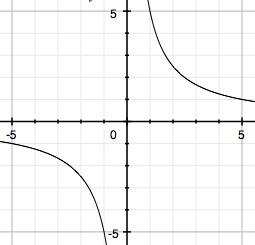
\includegraphics[width=\textwidth, height=14cm]{graph3}
\end{figure}	
	\chapter{Appendix 5 Title}
	\begin{figure}[h!]
	\centering
	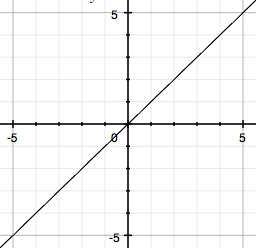
\includegraphics[width=\textwidth, height=14cm]{graph1}
\end{figure}	
\end{appendices}


\end{document}
